\section{Riassunto: Politiche dei servizi TCP/UDP}
\subsubsection{Servizio UDP:}
\begin{itemize}
    \item Scompone il flusso di byte in segmenti
    \item Li invia, uno per volta, ai servizi network
\end{itemize}
\subsubsection{Servizio TCP:}
\begin{itemize}
    \item Scompone e invia come UDP
    \item Ogni segmento viene numerato per garantire:
    \\• Riordinamento dei segmenti arrivati
    \\• Controllo delle duplicazioni (scarto i segmenti con ugual numero d'ordine)
    \\• Controllo delle perdite (rinvio i segmenti mancanti)
    \item Per progettare e realizzare sistemi distribuiti
    \\• NON è necessario conoscere il funzionamento (information hiding) dei processi
    \\• Ciò che importa è lo scambio dati (stream di byte) tra i processi
\end{itemize}

\section{Riassunto: Socket: funzionamento di base}
\subsubsection{TCP}
\begin{itemize}
    \item Utilizza variabili e buffer per realizzare il trasferimento bidirezionale di flussi di bytes (“pipe”) tra processi
    \item Prevede ruoli client/server durante la connessione
    \item NON prevede ruoli client/server per la comunicazione
    \item Utilizza i servizi dello strato IP per l'invio dei flussi di bytes
\end{itemize}
\subsubsection{API: Application Programming Interface}
\begin{itemize}
    \item Definisce l'interfaccia tra applicazione e strato di trasporto
\end{itemize}
\subsubsection{Socket: API per accedere a TCP e UDP}
Struttura usata per definire le comunicazioni
\begin{itemize}
    \item Due processi (applicazione nel modello client server) comunicano inviando/leggendo dati in/da socket
\end{itemize}

\section{Riassunto: Aspetti critici}
Gestione del ciclo di vita di client e server
\begin{itemize}
    \item Attivazione/terminazione del cliente e del server (es. Manuale o gestita da un middleware)
\end{itemize}
Identificazione e accesso al server
\begin{itemize}
    \item Informazioni che deve conoscere il cliente per accedere al server
\end{itemize}
Comunicazione tra cliente e server
\begin{itemize}
    \item Le primitive disponibili e le modalità per la comunicazione (es. TCP/IP: Stream di dati inviati con send/receive)
\end{itemize}
Ripartizione dei compiti tra i diversi componenti, in primo piano client e server
\begin{itemize}
    \item Dipende dal tipo di applicazione (es. controllo: una banca gestisce tutto lato server)
    \item Influenza la prestazioni in relazione al carico (numero di clienti)
\end{itemize}
Qua naming non c'è.

\section{Riassunto: Identificare il server}
Come fa quindi il client a conoscere l'indirizzo del server? O anche il nome della macchina e della porta?
\\Alternative:
\begin{itemize}
    \item inserire nel codice del client l'indirizzo del server espresso come costante (es. il client di un servizio bancario)
    \item chiedere all'utente l'indirizzo (es. web browser)
    \item utilizzare un name server o un repository da cui il client può acquisire le informazioni necessarie (es. Domain Name Service - DNS - per tradurre nomi simbolici)
    \item adottare un protocollo diverso per l'individuazione del server (es. broadcast per DHCP)
\end{itemize}

\section{Riassunto: Problemi e TCP/IP}
Come sono trattate le 4 problematiche fondamentali dei sistemi distribuiti con TCP e IP?
\\Sfruttiamo le 4 fasi tipiche che abbiamo già visto e previste per identificare ogni nuova tecnologia che ci troviamo davanti:
\begin{description}
    \item[Identifico la controparte (naming):] identificazione di basso livello, nome degli hosts e dei protocolli
    \item[Accedo alla controparte (access point):] uso dell'indirizzo IP (host:port) per accedere ad un processo
    \item[Comunicazione 1 (protocollo):] stream di bytes
    \item[Comunicazione 2 (sintassi e semantica):] protocolli applicativi con semantiche predefinite (http, smtp)
    \item[What level of transparency?] Molto basso: il programmatore/l'utente deve
    \item[] - conoscere l'indirizzo di rete
    \item[] - fare il parsing di bytes per accedere al contenuto (messaggio)
\end{description}

\textbf{IMPORTANTE}: TCP si può usare per qualsiasi tipo di comunicazione? Perché non c'è semantica. Quindi il punto di Comunicazione 2 non c'è. \textbf{Questa potrebbe essere una domanda dell'esame}.

\section{Riassunto: Comunicazione via socket}
La comunicazione TCP/IP avviene attraverso flussi di byte (byte stream), dopo una connessione esplicita, tramite normali \textbf{\textit{system call} read/write}.
\\Read e write:
\begin{itemize}
    \item Sono sospensive (bloccano il processo finché il sistema operativo non ha effettuato la lettura/scrittura) --> sistema-bloccanti
    \item Utilizzano un buffer per garantire flessibilità (es: la read definisce un buffer per leggere N caratteri, ma potrebbe ritornare avendone letti solo $\text{k}<\text{N}$)
\end{itemize}
\begin{center}
    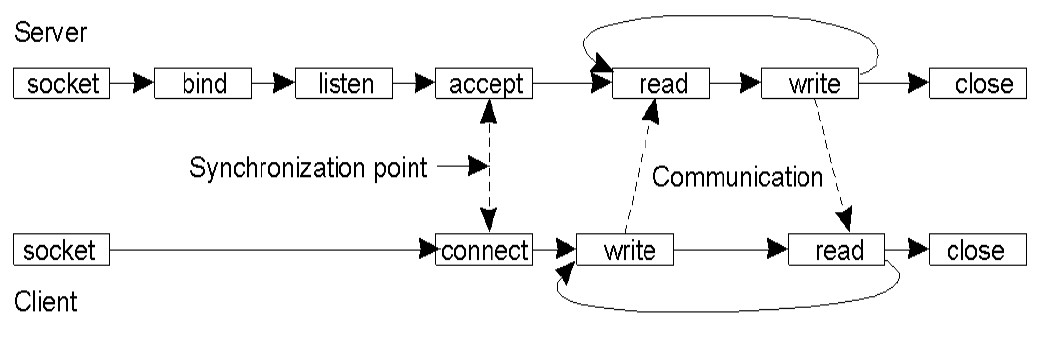
\includegraphics[width=0.75\textwidth]{img/socket_comunicazione1.jpg}
\end{center}
N.B. importante: due cose e me ne sono persa una.
\begin{itemize}
    \item \textbf{le system call sono sistema-bloccanti}
    \item ho read e write. Sono system calls ma pur sempre read e write, è il protocollo che uso che ne decide l'ordine. Ma è sempre "client-server"
\end{itemize}
Client e server prima di avviare la comunicazione devono \textbf{concordare} su un protocollo. Questo protocollo si occuperà di definire read e write (l'ultima è quella che effettivamente mi definisce la quantità di informazione con cui lavoro). 

\section{Riassunto: API socket system calls (Berkeley)}
Questo è un po' un riassunto di quanto detto finora.
\\Molte chiamate sono previste per accedere ai servizi TCP e UDP.
\\Le più importanti nella tabella seguente:
\begin{center}
    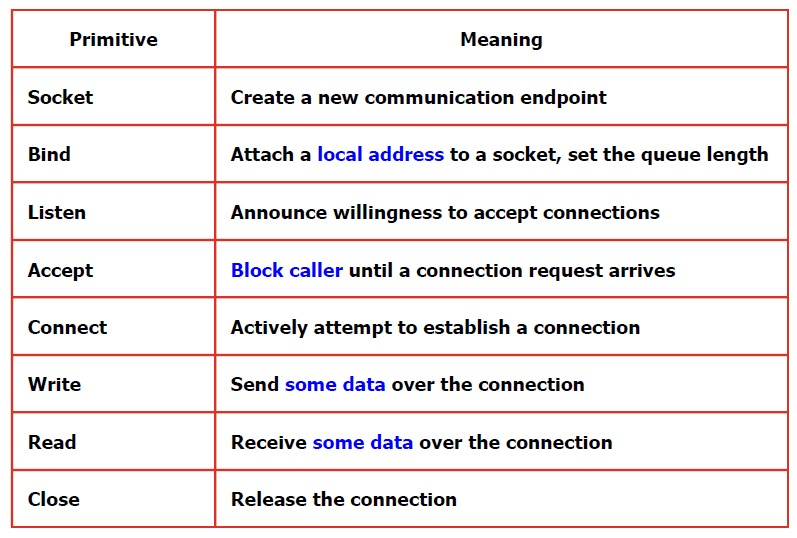
\includegraphics[width=0.75\textwidth]{img/berkeley1.jpg}
\end{center}

\section{Processi e socket}
Il server crea una socket collegata alla well-known port (che identifica il servizio fornito) dedicata a ricevere richieste di connessione.
\\Con la accept(), il server crea una nuova socket, cioè un nuovo canale, dedicato alla comunicazione con il client.
\begin{center}
    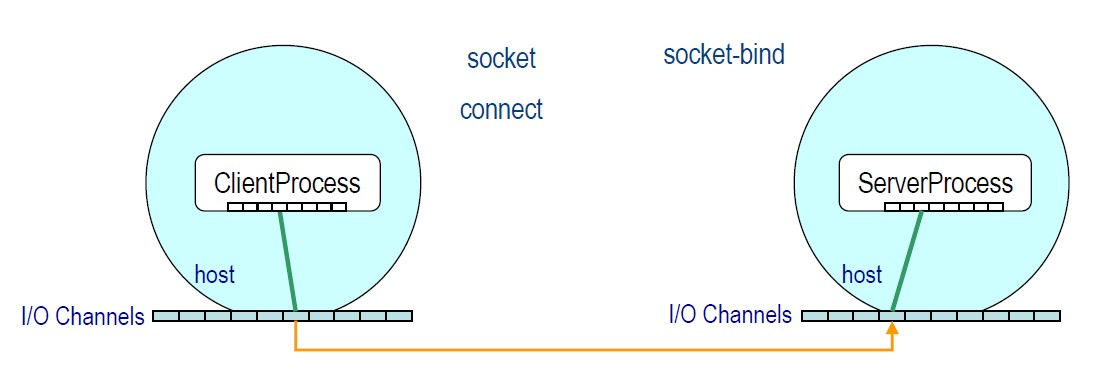
\includegraphics[width=0.75\textwidth]{img/processi_e_socket2.jpg}
\end{center}
Domanda: Chi stabilisce il formato della richiesta? L'applicazione o lo strato di trasporto (TCP)?
\\Ovviamente il protocollo. Ma dove avviene la connect? A livello di servizio, l'applicazione (qualunque essa sia) avviene da lì a destra (si occupa di read e write). Perciò la risposta è: \textit{a livello di trasporto}.
\\Si genera una seconda domanda: Perché non si usa la stessa socket?
\begin{center}
    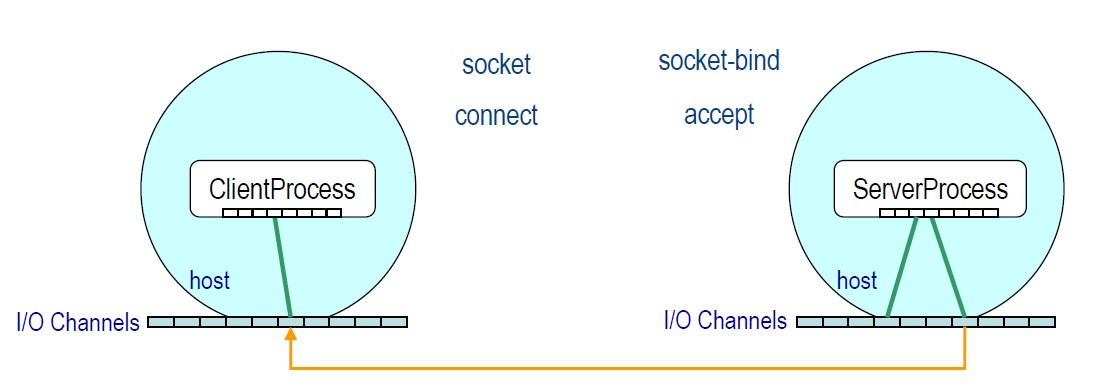
\includegraphics[width=0.75\textwidth]{img/processi_e_socket3.jpg}
\end{center}
Giriamo la domanda: \textbf{potrei} usare la stessa socket? 
\\Sì, ma mi servirebbe un canale distinto per identificare i bit dell'indirizzo e quelli dell'informazione della comunicazione (parliamo di \textbf{programmazione strutturale}). Nel caso di uno stream, non sarei in grado di discriminare. Diventa complicato.
\\L'altro tipo di programmazione, p. dinamica, fa tutto lei invece di compartimentalizzare come fa la p. strutturale che abbiamo appena analizzato. La \textit{programmazione dinamica} è più soggetta ad errori di quella \textit{strutturale}.
\begin{center}
    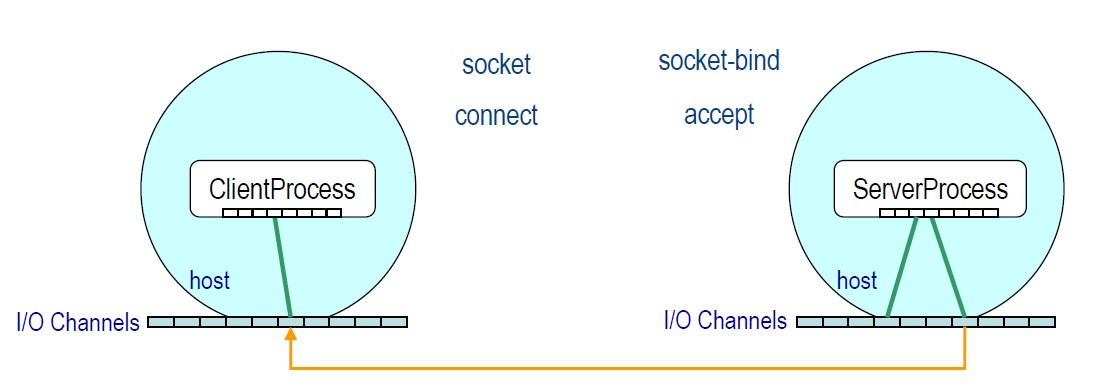
\includegraphics[width=0.75\textwidth]{img/processi_e_socket3.jpg}
\end{center}

\section{Read e write}
Le socket trasportano “stream” (= flussi) di bytes, quindi
\begin{itemize}
    \item \textit{non c'è il concetto di “messaggio”} (il flusso è continuo, senza fine),
    \item \textit{la lettura/scrittura avviene per un numero \textbf{arbitrario} di byte}
\end{itemize}
Il prototipo (in pseudocodice) della read è quindi
\\byteLetti read(socket, buffer, dimBuffer);
\\byteLetti = byte effettivamente letti
\\socket = il canale da cui leggere
\\buffer = lo spazio di memoria dove trasferire i byte letti
\\dimBuffer = dimensione del buffer = numero max di caratteri che si possono leggere
\\
\\\textbf{Quindi si devono prevedere cicli di lettura che termineranno in base alla dimensione dei “messaggi” come stabilito dal formato del protocollo applicativo in uso}.

% NB ha detto che la read è una system call, ed è NELL'applicazione. Io mi sto perdendo malissimo.

Ovviamente quella read lì definita va in un while per passare tutta l'informazione.

\chapter{Le socket in Java}
Java definisce alcune classi che costituiscono un'interfaccia ad oggetti alle system call illustrate in precedenza. Ricorda che Java nasconde la gestione della memoria (e garbage collector) ma all'interno avviene come illustrato nella sezione precedente.
\\Le principali:
\begin{itemize}
    \item java.net.Socket
    \item java.net.ServerSocket
\end{itemize}
Queste \textbf{classi} accorpano funzionalità e mascherano alcuni dettagli con il vantaggio di semplificarne l'uso.
\\Come per ogni framework è necessario conoscerne il modello e il funzionamento per poterlo utilizzare in modo efficace.
\\Le prossime slide discutono i principali metodi delle due classi. SONO DA SISTEMARE

\section{java.net.Socket}
\subsubsection{Constructors}
\begin{description}
    \item[public Socket()] 
\end{description}
Creates an unconnected socket, with the system-default type of SocketImpl.
public Socket(String host, int port)
throws UnknownHostException, IOException
Creates a stream socket and connects it to the specified port number on the named host. If the specified host is null, the
loopback address is assumed.
The UnknownHostException is thrown if the IP address of the host could not be determined.
public Socket(InetAddress address, int port)
throws IOException
Creates a stream socket and connects it to the specified port number at the specified IP address.
\subsubsection{Methods to manage connections}
public void bind(SocketAddress bindpoint) throws IOException
Binds the socket to a local address. If the address is null, then the system will pick up an ephemeral port and a valid local address
to bind the socket.
public void connect(SocketAddress endpoint) throws IOException
Connects this socket to the server.
public void connect(SocketAddress endpoint, int timeout)
throws IOException
Connects this socket to the server with a specified timeout value (in milliseconds).
public void close()
Closes this socket.
\\Sono tutte bloccanti queste chiamate.
Methods to establish I/O channels to exchange bytes
public InputStream getInputStream() throws IOException
Returns an input stream for this socket.
If this socket has an associated channel then the resulting input stream delegates all of its operations to the channel.
If the channel is in non-blocking mode then the input stream's read operations will throw an
IllegalBlockingModeException.
When a broken connection is detected by the network software the following applies to the returned input stream:
• The network software may discard bytes that are buffered by the socket. Bytes that aren't discarded by the
network software can be read using read.
• If there are no bytes buffered on the socket, or all buffered bytes have been consumed by read, then all
subsequent calls to read will throw an IOException.
• If there are no bytes buffered on the socket, and the socket has not been closed using close, then available
will return 0.
public OutputStream getOutputStream() throws IOException
Returns an output stream for writing bytes to this socket.
If this socket has an associated channel, then the resulting output stream delegates all of its operations to the
channel.
If the channel is in non-blocking mode, then the output stream's write operations will throw an
IllegalBlockingModeException.

\section{java.net.ServerSocket}
\subsubsection{Constructors}
public ServerSocket() throws IOException
Creates an unbound server socket.
public ServerSocket(int port) throws IOException
Creates a server socket, bound to the specified port.
A port of 0 creates a socket on any free port.
The maximum queue length for incoming connection indications (a request to connect) is set to 50.
If a connection indication arrives when the queue is full, the connection is refused.
public ServerSocket(int port, int backlog) throws IOException
Creates a server socket and binds it to the specified local port number, with the specified backlog.
A port of 0 creates a socket on any free port.
The maximum queue length for incoming connection indications (a request to connect) is set to the backlog
parameter.
If a connection indication arrives when the queue is full, the connection is refused.
\subsubsection{Methods to manage connections}
public void bind(SocketAddress endpoint) throws IOException
Binds the ServerSocket to a specific address (IP address and port number).
If the address is null, then the system will pick up an ephemeral port and a valid local address to bind the socket.
public void bind(SocketAddress endpoint, int backlog) throws IOException
Binds the ServerSocket to a specific address (IP address and port number).
If the address is null, then the system will pick up an ephemeral port and a valid local address to bind the socket.
The backlog argument must be a positive value greater than 0. If the value passed if equal or less than 0, then the
default value will be assumed.
public Socket accept() throws IOException
Listens for a connection to be made to this socket and accepts it. Returns the new Socket.
The method blocks until a connection is made.
\subsubsection{Utility methods}
public InetAddress getInetAddress()
Returns the local address of this server socket or null if the socket is unbound.
public int getLocalPort()
Returns the port on which this socket is listening or -1 if the socket is not bound yet.
public SocketAddress getLocalSocketAddress()
Returns the address of the endpoint this socket is bound to, or null if it is not bound yet.

\subsection{Un esempio}
Let's study an example in which:
\begin{itemize}
    \item A server accept a connection with a client, and then sends a stream of bytes (e.g., a string of characters)
    \item A client request a connection, and then reads the stream of bytes sent by the server
\end{itemize}
The goal is to give evidence that:
\begin{itemize}
    \item The behavior of the involved processes is independent from each other
    \item They exchange streams of byte 
    \item The notion of “message” or “application protocol” is not part of the socket definition
\end{itemize}

\subsubsection{Sender Server Socket}
\begin{center}
    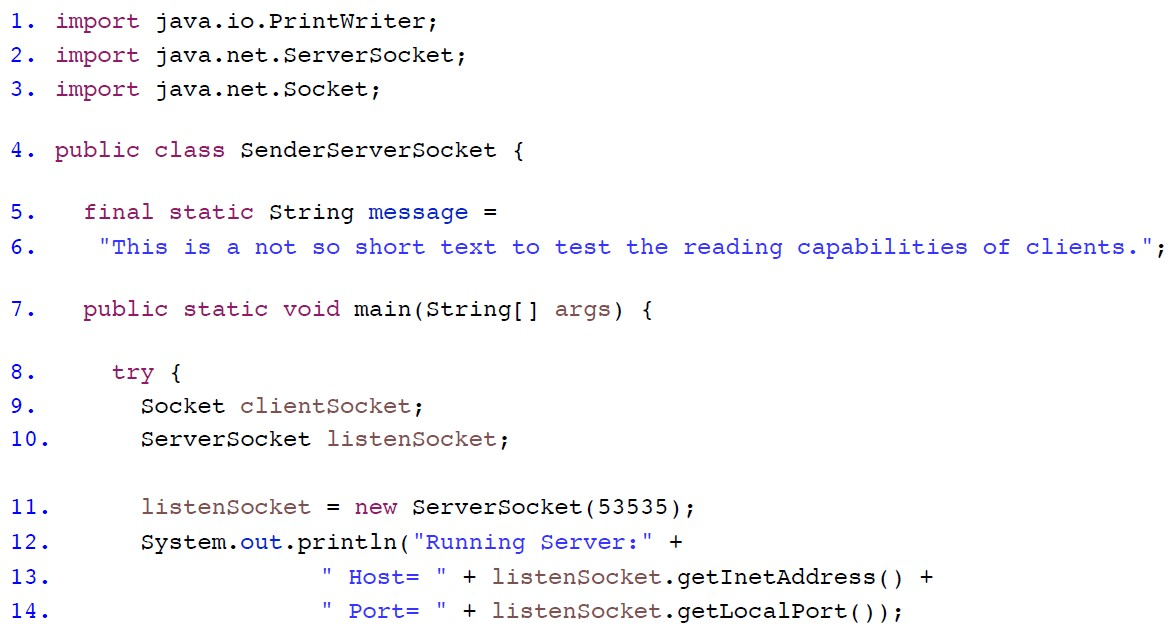
\includegraphics[width=0.75\textwidth]{img/SenderServerSocket1.jpg}
\end{center}
\begin{center}
    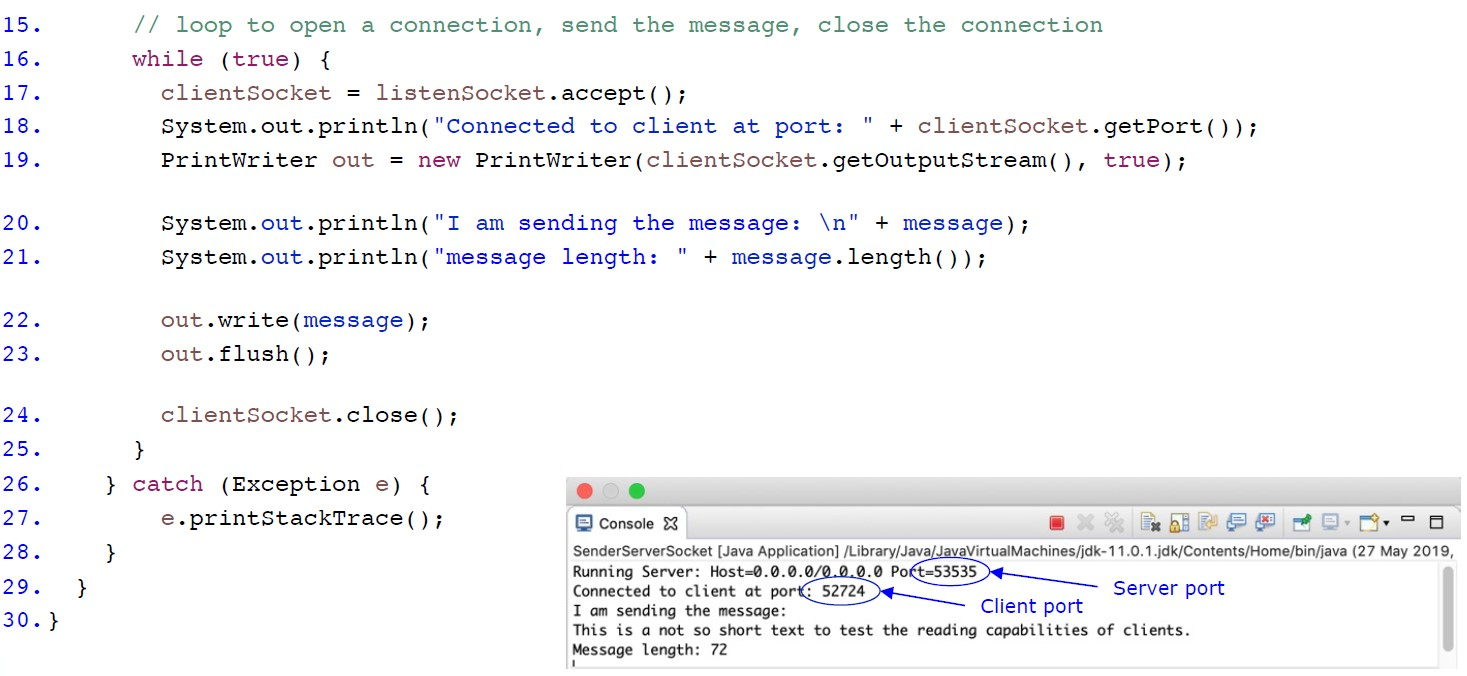
\includegraphics[width=0.75\textwidth]{img/SenderServerSocket2.jpg}
\end{center}

\subsubsection{Receiver Client Socket}
Nella slide seguente è possibile vedere un parser: serve perché i caratteri immessi sono char e stringhe.
\begin{center}
    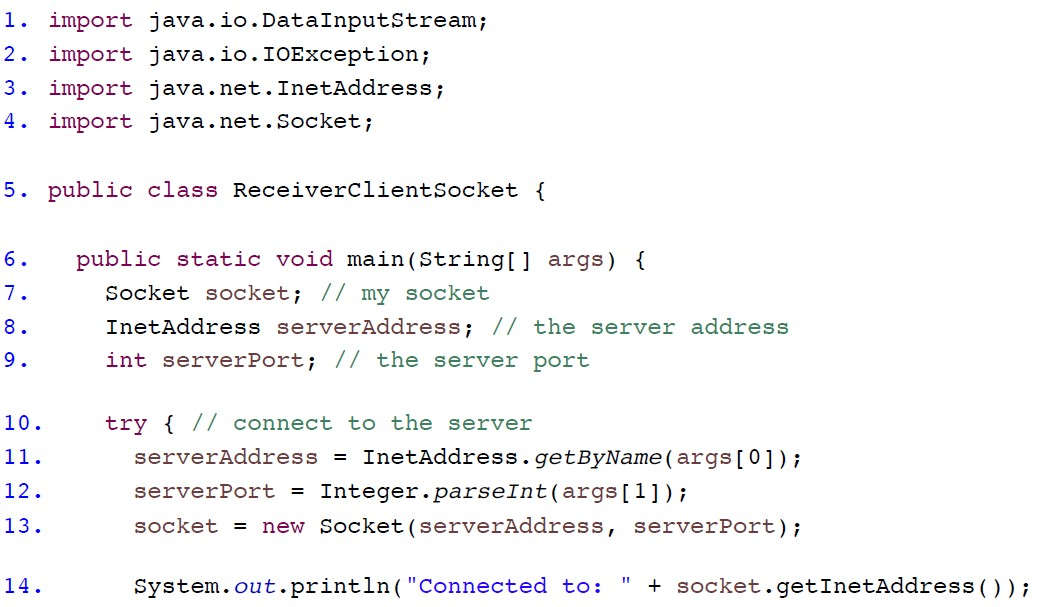
\includegraphics[width=0.75\textwidth]{img/ReceiverClientSocket1.jpg}
\end{center}
\begin{center}
    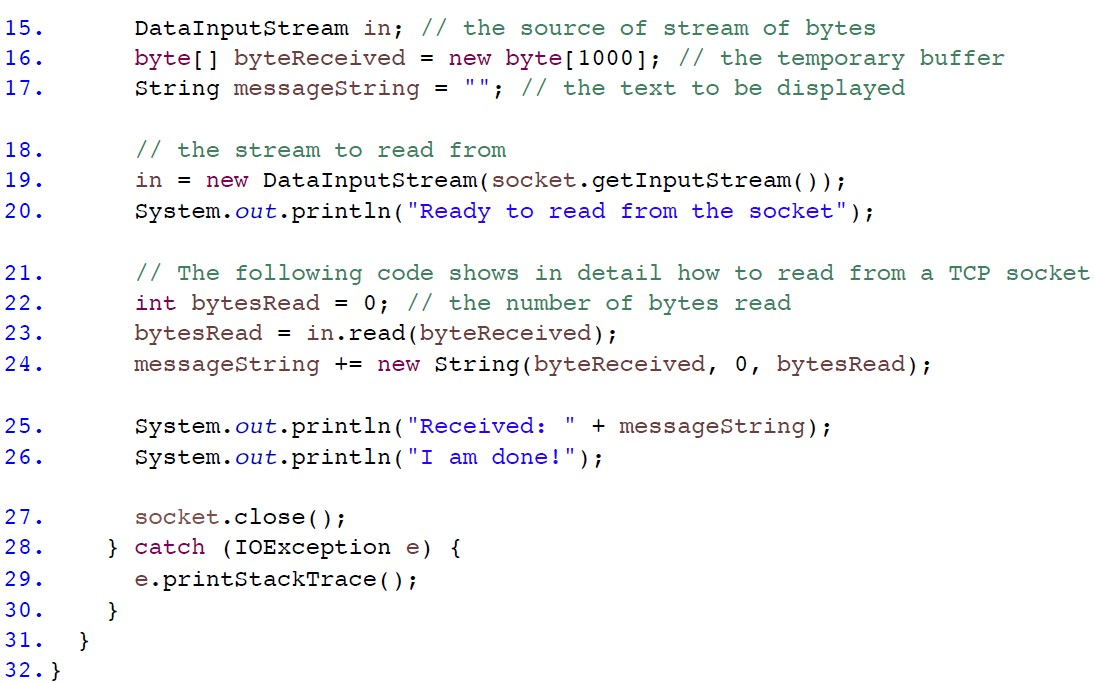
\includegraphics[width=0.75\textwidth]{img/ReceiverClientSocket2.jpg}
\end{center}

\subsubsection{Esecuzione}
\begin{center}
    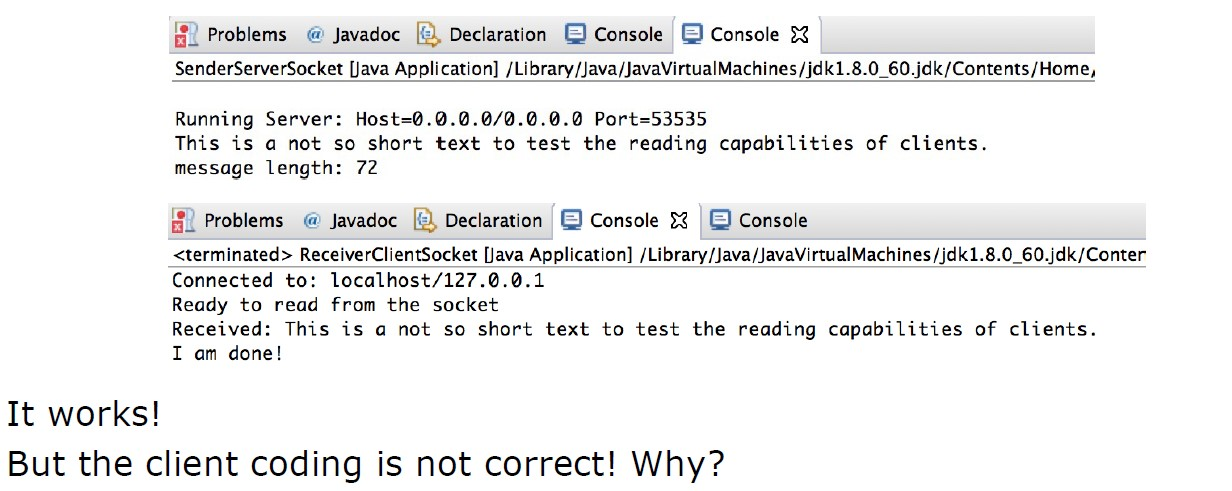
\includegraphics[width=0.75\textwidth]{img/esecuzione_es_SSS_RCS1.jpg}
\end{center}
To discover the answer, let's introduce the Lazy Server: it's a server that sends a few bytes at a time (9 a 9) with a delay between sendings.

\subsubsection{Lazy Sender Server Socket}
\begin{center}
    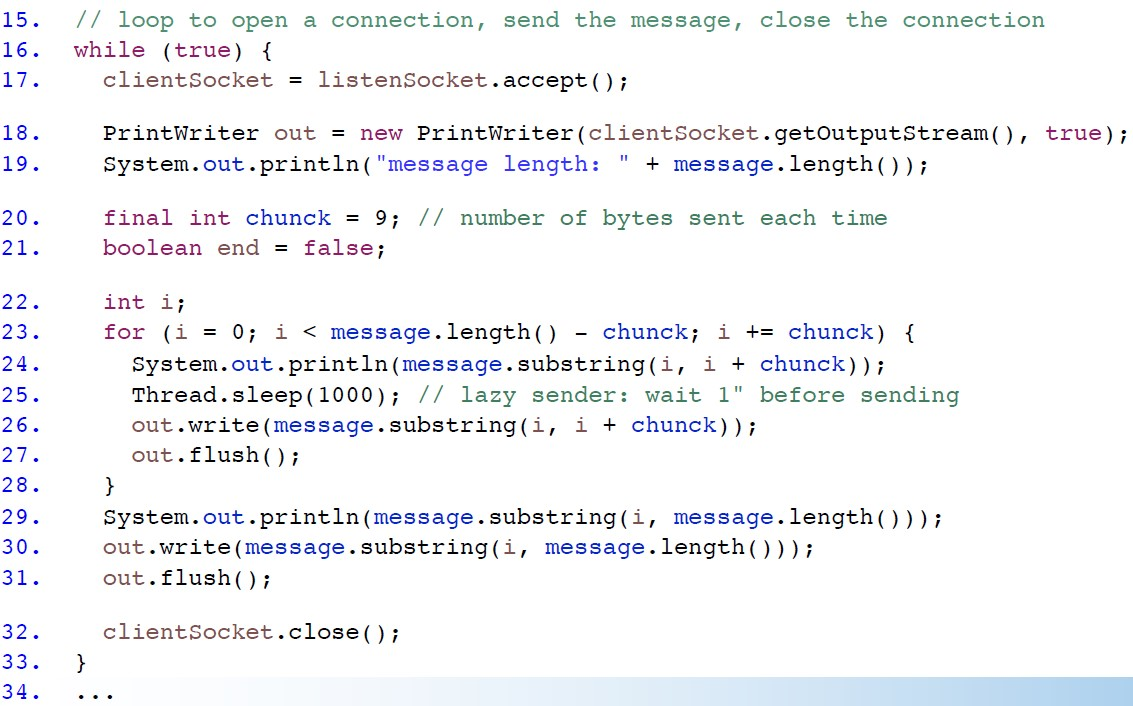
\includegraphics[width=0.75\textwidth]{img/LazySenderServerSocket1.jpg}
\end{center}
\begin{center}
    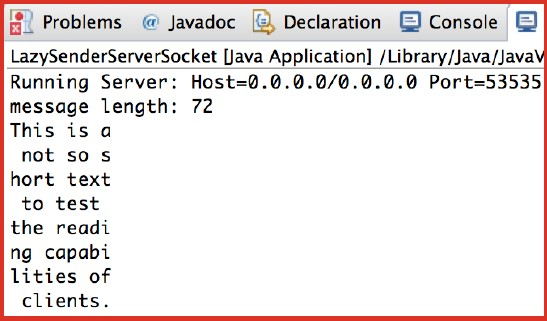
\includegraphics[width=0.75\textwidth]{img/LazySenderServerSocket2.jpg}
\end{center}

\subsubsection{Receiver Client Socket execution}
\begin{center}
    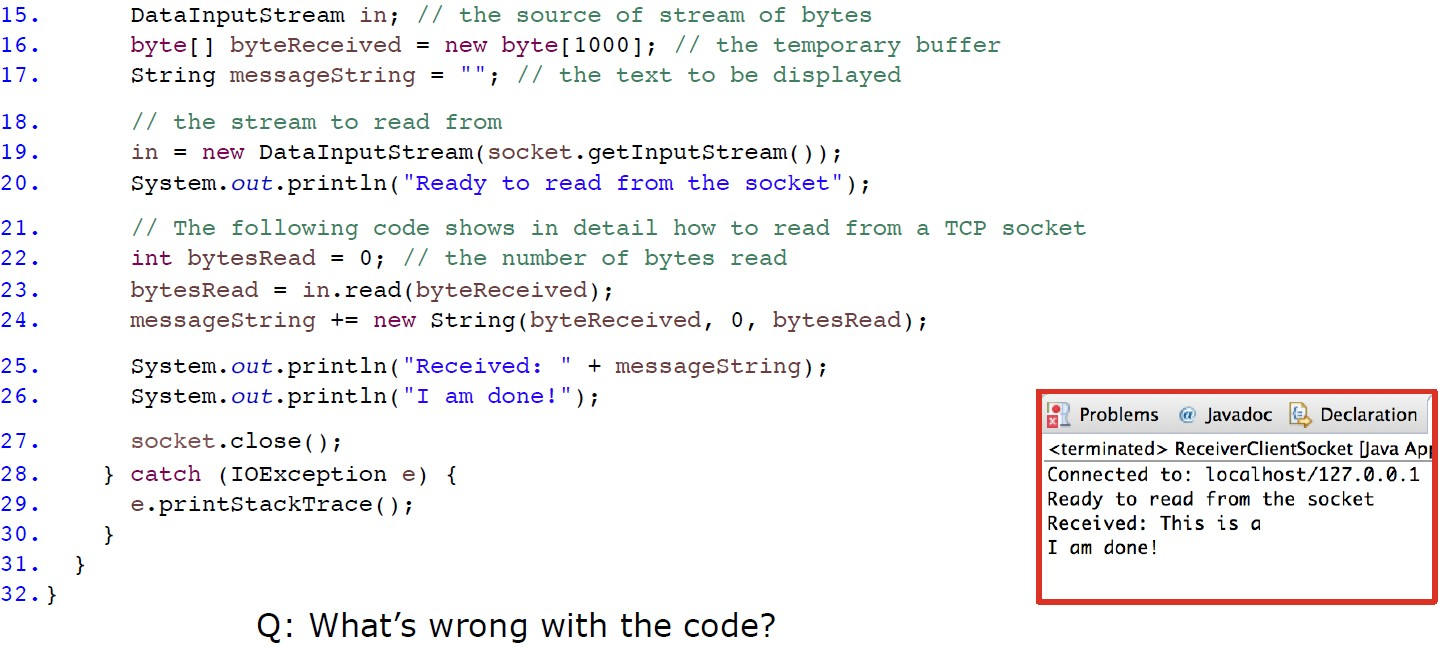
\includegraphics[width=0.75\textwidth]{img/LazySenderServerSocket3.jpg}
\end{center}

\section{Progettare un'applicazione con le socket}
\begin{description}
    \item[Client:] L'architettura è concettualmente più semplice di quella di un server
    \item[] • È spesso un'applicazione convenzionale che usa una socket anziché da un altro canale I/O
    \item[] • Ha effetti solo sull'utente client: non ci sono particolari problemi di sicurezza
    \item[Server:] L'architettura generale prevede che
    \item[] • venga creata una socket con una porta nota per accettare le richieste di connessione
    \item[] • entri in un ciclo infinito in cui alternare:
    \\1. attesa/accettazione di una richiesta di connessione da un client
    \\2. ciclo lettura-esecuzione, invio risposta fino al termine della conversazione (stabilito spesso dal client)
    \\3. chiusura connessione
\end{description}
Problematiche connesse:
\begin{itemize}
    \item L'affidabilità del server è strettamente dipendente dall'affidabilità della comunicazione tra lui e i suoi client
    \item La modalità connection-oriented determina:
    \\• l'impossibilità di rilevare interruzioni sulle connessioni (il client controlla il server) che potrebbero essere intromissioni esterne o problemi sulla rete;
    \\• la necessità di una connessione (una socket) per ogni conversazione;
    \\• problemi di sicurezza per la condivisione dei dati e il controllo affidato al client.
\end{itemize}

\chapter{Architetture dei server}
\section{Tipi di server}
I server possono essere:
\begin{description}
    \item[iterativi:] soddisfano una richiesta alla volta
    \item[concorrenti processo singolo:] simulano la presenza di un server dedicato
    \item[concorrenti multi-processo:] creano server dedicati
    \item[concorrenti multi-thread:] creano thread dedicati
\end{description}

\section{Progettare un server iterativo}
Al momento di una richiesta di connessione il server crea una socket temporanea per stabilire una connessione diretta con il client.
\\Le eventuali ulteriori richieste per il server verranno accodate alla porta nota per essere successivamente soddisfatte.
\\Vantaggi:
\begin{itemize}
    \item Semplice da progettare
\end{itemize}
Svantaggi:
\begin{itemize}
    \item Viene servito un cliente alla volta, gli altri devono attendere
    \item Un client può impedire l'evoluzione di altri client
    \item Non scala
\end{itemize}
Soluzione: server concorrenti
\begin{center}
    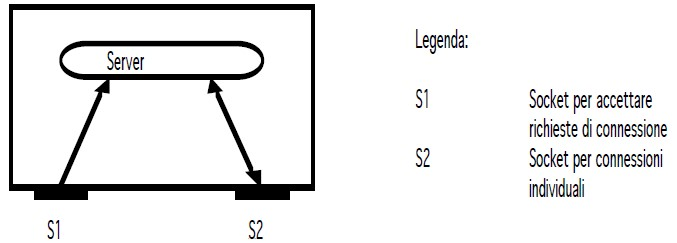
\includegraphics[width=0.75\textwidth]{img/serverIterativi1.jpg}
\end{center}

Manca una slide

\section{Progettare un server concorrente}
Un server concorrente può gestire più connessioni client.
\\La sua realizzazione può essere
\begin{itemize}
    \item simulata con un solo processo \textbf{(A)} in C: funzione select, in Java: uso Selector
che conoscere i canali ready to use
(B) in Java: uso dei Thread
• reale creando nuovi processi slave
(C) in C: uso della funzione fork
\end{itemize}


\begin{center}
    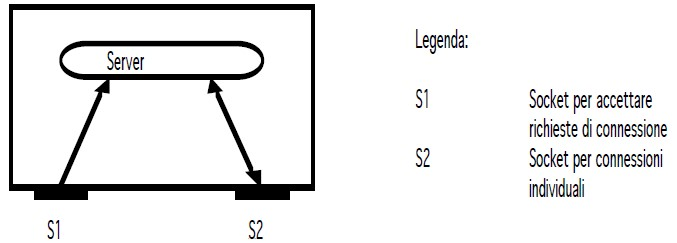
\includegraphics[width=0.75\textwidth]{img/serverIterativi1.jpg}
\end{center}

\begin{center}
    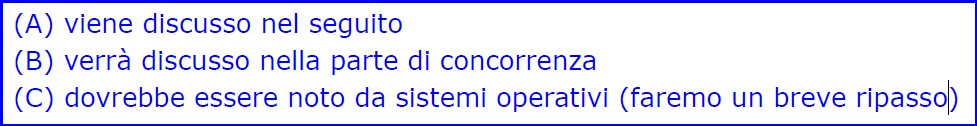
\includegraphics[width=0.75\textwidth]{img/dacanc1.jpg}
\end{center}

Manca una slide

% in B ho un sotto processo --> questo vuol dire un sistema di controllo autonomo

